\documentclass[10pt,xcolor=svgnames,pdflatex]{beamer}
\usepackage{newcent}
\usepackage[utf8]{inputenc}
%\usepackage[czech]{babel}
\usepackage{biblatex}
\usepackage{hyperref}
\usepackage{fancyvrb}
\usepackage{float}

\usepackage{tikz}
\usetikzlibrary{decorations.markings}
\usetikzlibrary{shapes.geometric}

\pgfdeclarelayer{edgelayer}
\pgfdeclarelayer{nodelayer}
\pgfsetlayers{edgelayer,nodelayer,main}

\tikzstyle{none}=[inner sep=0pt]

\tikzstyle{rn}=[circle,fill=Red,draw=Black,line width=0.8 pt]
\tikzstyle{gn}=[circle,fill=Lime,draw=Black,line width=0.8 pt]
\tikzstyle{yn}=[circle,fill=Yellow,draw=Black,line width=0.8 pt]

\tikzstyle{simple}=[-,draw=black,line width=2.000]
\tikzstyle{arrow}=[-,draw=black,postaction={decorate},decoration={markings,mark=at position .5 with {\arrow{>}}},line width=2.000]
\tikzstyle{tick}=[-,draw=black,postaction={decorate},decoration={markings,mark=at position .5 with {\draw (0,-0.1) -- (0,0.1);}},line width=2.000]
\tikzstyle{newstyle}=[->,draw=black,line width=2.000]

\usepackage{tikz-qtree}


\usetheme{FIT}

\usetikzlibrary{arrows,backgrounds,shadows, positioning}
\bibliography{prezentace.bib}

\pgfdeclarelayer{edgelayer}
    \pgfdeclarelayer{nodelayer}
% tell TikZ how to stack them (back to front)
    \pgfsetlayers{nodelayer,main,edgelayer}

%%%%%%%%%%%%%%%%%%%%%%%%%%%%%%%%%%%%%%%%%%%%%%%%%%%%%%%%%%%%%%%%%%
\title[strace2seccomp]{Automatic Seccomp Syscall\\Policy Generator}

\author[]{Marek Tamaskovic}

\institute[]{Brno University of Technology, Faculty of Information Technology\\
Bo\v{z}et\v{e}chova 1/2. 612 66 Brno - Kr\'alovo Pole\\
xtamas01@fit.vutbr.cz}

\date{August 22, 2018}
%\date{\today}
%\date{} % bez data

%%%%%%%%%%%%%%%%%%%%%%%%%%%%%%%%%%%%%%%%%%%%%%%%%%%%%%%%%%%%%%%%%%

\begin{document}

\frame[plain]{\titlepage}

\begin{frame}\frametitle{Introduction}

\begin{columns}
  \begin{column}{0.6\textwidth}
     \begin{itemize}
       \item Ing. Lenka Turo\v{n}ov\'a
       \item Bc. Daniel Kope\v{c}ek
       \item Cooperation with RedHat Inc.\\
       \item Motivation?
     \end{itemize}
  \end{column}
  \begin{column}{0.4\textwidth}
      \begin{center}
        
\includegraphics[width=1\textwidth]{img/Logo_RH_BW_RGB}
      \end{center}
  \end{column}
\end{columns}

\end{frame}

\begin{frame}\frametitle{Input / Output}
    \begin{columns}
        \begin{column}{0.5\textwidth}
          Input:
          \begin{itemize}
            \item \emph{strace} log
          \end{itemize}
        \end{column}
        \begin{column}{0.5\textwidth}
          Output:
          \begin{itemize}
            \item C\textbackslash C++ code template
            \item \emph{libseccomp}
          \end{itemize}
        \end{column}
    \end{columns}
    \vfill
    \begin{figure}[]
	  \centering
	  % \includestandalone[]{obrazky-figures/mytikz}%     without .tex extension
	  \resizebox {0.5\textwidth} {!} {
	    \input{img/files.tikz}
	  }
	  \caption{Transforamtion}
	  \label{fig:tikz:transformation}
	\end{figure}
\end{frame}

\begin{frame}\frametitle{Architecture}
  \begin{figure}[h]
  \centering
  \resizebox {\textwidth} {!} {
    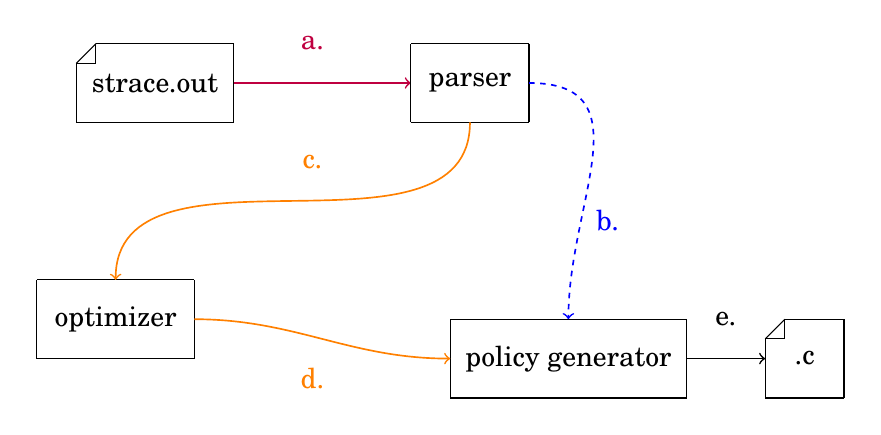
\begin{tikzpicture}
	\begin{pgfonlayer}{nodelayer}
		\node [] (0) at (-6.75, 6) {};
		\node [] (1) at (-6.75, 5) {};
		\node [] (2) at (-8.75, 5) {};
		\node [] (3) at (-6.75, 5.5) {};
		\node [] (4) at (-4.5, 5.5) {};
		\node [] (5) at (-4.5, 6) {};
		\node [] (6) at (-4.5, 5) {};
		\node [] (7) at (-3, 5) {};
		\node [] (8) at (-3, 6) {};
		\node [] (9) at (-9.25, 3) {};
		\node [] (10) at (-7.25, 3) {};
		\node [] (11) at (-7.25, 2) {};
		\node [] (12) at (-9.25, 2) {};
		\node [] (13) at (-8.25, 2.5) {optimizer};
		\node [] (14) at (-4, 2.5) {};
		\node [] (15) at (-4, 1.5) {};
		\node [] (16) at (-1, 2.5) {};
		\node [] (17) at (-1, 1.5) {};
		\node [] (18) at (-2.5, 2) {policy generator};
		\node [] (19) at (-2.5, 2.5) {};
		\node [] (20) at (-4, 2) {};
		\node [] (21) at (-3.75, 5) {};
		\node [] (22) at (-8.25, 3) {};
		\node [] (23) at (-7.25, 2.5) {};
		\node [] (24) at (-3, 5.5) {};
		\node [] (25) at (-7.75, 5.5) {strace.out};
		\node [] (26) at (0, 1.5) {};
		\node [] (27) at (1, 1.5) {};
		\node [] (28) at (1, 2.5) {};
		\node [] (29) at (0.5, 2) {.c};
		\node [] (30) at (0, 2) {};
		\node [] (31) at (-1, 2) {};
		\node [] (32) at (-3.75, 5.5) {parser};
		\node [style={color=blue}] (33) at (-2, 3.75) {b.};
		\node [style={color=purple}] (34) at (-5.75, 6) {a.};
		\node [style={color=orange}] (35) at (-5.75, 4.5) {c.};
		\node [style={color=orange}] (36) at (-5.75, 1.75) {d.};
		\node [] (37) at (0, 2.25) {};
		\node [] (38) at (0.25, 2.5) {};
		\node [] (39) at (-8.75, 5.75) {};
		\node [] (40) at (-8.5, 6) {};
		\node [] (41) at (0.25, 2.25) {};
		\node [] (42) at (-8.5, 5.75) {};
		\node [] (43) at (-0.5, 2.5) {e.};
	\end{pgfonlayer}
	\begin{pgfonlayer}{edgelayer}
		\draw (20.center) to (15.center);
		\draw (15.center) to (17.center);
		\draw (16.center) to (19.center);
		\draw (19.center) to (14.center);
		\draw (14.center) to (20.center);
		\draw (11.center) to (12.center);
		\draw (12.center) to (9.center);
		\draw (2.center) to (1.center);
		\draw (1.center) to (3.center);
		\draw (3.center) to (0.center);
		\draw [semithick, color=purple, ->] (3.center) to (4.center);
		\draw (4.center) to (5.center);
		\draw (5.center) to (8.center);
		\draw (6.center) to (4.center);
		\draw (6.center) to (21.center);
		\draw (21.center) to (7.center);
		\draw (9.center) to (22.center);
		\draw (22.center) to (10.center);
		\draw [semithick, color=orange, <-, in=-90, out=90, looseness=1.00] (22.center) to (21.center);
		\draw (10.center) to (23.center);
		\draw (23.center) to (11.center);
		\draw [semithick, color=orange, ->, in=180, out=0, looseness=1.00] (23.center) to (20.center);
		\draw (8.center) to (24.center);
		\draw (24.center) to (7.center);
		\draw [semithick, color=blue, dash pattern=on 2pt off 2pt, ->, in=90, out=0, looseness=1.25] (24.center) to (19.center);
		\draw (28.center) to (27.center);
		\draw (27.center) to (26.center);
		\draw (30.center) to (26.center);
		\draw (16.center) to (31.center);
		\draw (31.center) to (17.center);
		\draw [semithick, ->] (31.center) to (30.center);
		\draw (40.center) to (39.center);
		\draw (39.center) to (2.center);
		\draw (40.center) to (0.center);
		\draw (38.center) to (37.center);
		\draw (37.center) to (30.center);
		\draw (38.center) to (28.center);
		\draw (38.center) to (41.center);
		\draw (37.center) to (41.center);
		\draw (40.center) to (42.center);
		\draw (42.center) to (39.center);
	\end{pgfonlayer}
\end{tikzpicture}

  }
  \caption{Pipe\&Filter Architecture}
  \label{fig:tikz:architecture}
\end{figure}
\end{frame}

\begin{frame}\frametitle{Optimiziations}

  \begin{itemize}
    \item Three optimization levels
     \begin{itemize}
	    \item \emph{Strict}:
	    \begin{itemize}
	      \item 1:1
	      \item input $\rightarrow$ output
	    \end{itemize}
	    \item \emph{MinMax}:
	    \begin{itemize}
	      \item allowed intervals
	      \item border values are extremes
	    \end{itemize}
	    \item \emph{DBSCAN}\footnote{Density-based spatial clustering of applications with noise}:
	    \begin{itemize}
	      \item implemented DBSCAN\cite{Mahesh_Kumar2016, Schubert:2017:DRR:3129336.3068335}
	    \end{itemize}
	  \end{itemize}
  \end{itemize}

 
\end{frame}

\begin{frame}\frametitle{What have I achieved?}
    \begin{itemize}
    	\item Designed program architecture
    	\item Implemented:
    	\begin{itemize}
    		\item \emph{IDS}\footnote{Intermediate Data Structure}
    		\item 3 algorithms
    	\end{itemize}
    	\item Created \emph{testsuite}
    	\item \textit{"It is on good way to appear in production"}
    	\item $\sim$ 2.8K LOC\footnote{Lines of Code} + 
    \end{itemize}
\end{frame}

\begin{frame}\frametitle{Planed Extensions}
  \begin{itemize}
    \item \emph{Go} support
    \item \emph{ASLR}\footnote{Address Space Layout Randomization} turned off
    \item Customizable template
    \item Packaging
    \item More algorithms
  \end{itemize}
\end{frame}

\begin{frame}[allowframebreaks]
	\frametitle{References}
	\printbibliography
\end{frame}

\bluepage{Any questions?}

\appendix

\begin{frame}\frametitle{Question for defense}
    Název vašeho algoritmu je Minmax nebo Minimax? (V BP je toto nekonzistentní, i ve zdrojových kódech). Dokážete vysvětlit rozdíl oproti existujícímu algoritmu Minimax?
\end{frame}

\begin{frame}\frametitle{Inner Representation}
  \begin{figure}[h]
  \centering
  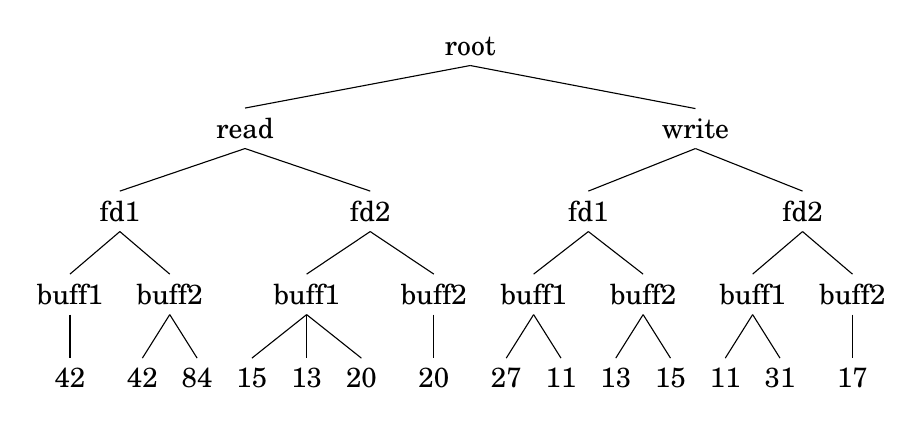
\begin{tikzpicture}
  \Tree [.root
          [.read
            [.fd1
              [.buff1 42 ]
              [.buff2 42 84 ]
            ]
            [.fd2
              [.buff1 15 13 20 ]
              [.buff2 20 ]
            ]
          ]
          [.write
            [.fd1
              [.buff1 27 11 ]
              [.buff2 13 15 ]
            ]
            [.fd2
              [.buff1 11 31 ]
              [.buff2 17 ]
            ]
          ]
        ]
  \end{tikzpicture}
  % \caption{Visualized IDS as a tree}
  \label{fig:tikz:IDStree}
\end{figure}
\end{frame}

\end{document}
